\subsection{Le diagramme de classe}
\label{subsec:class-diagram}

\begin{figure}[ht]
    \centering
    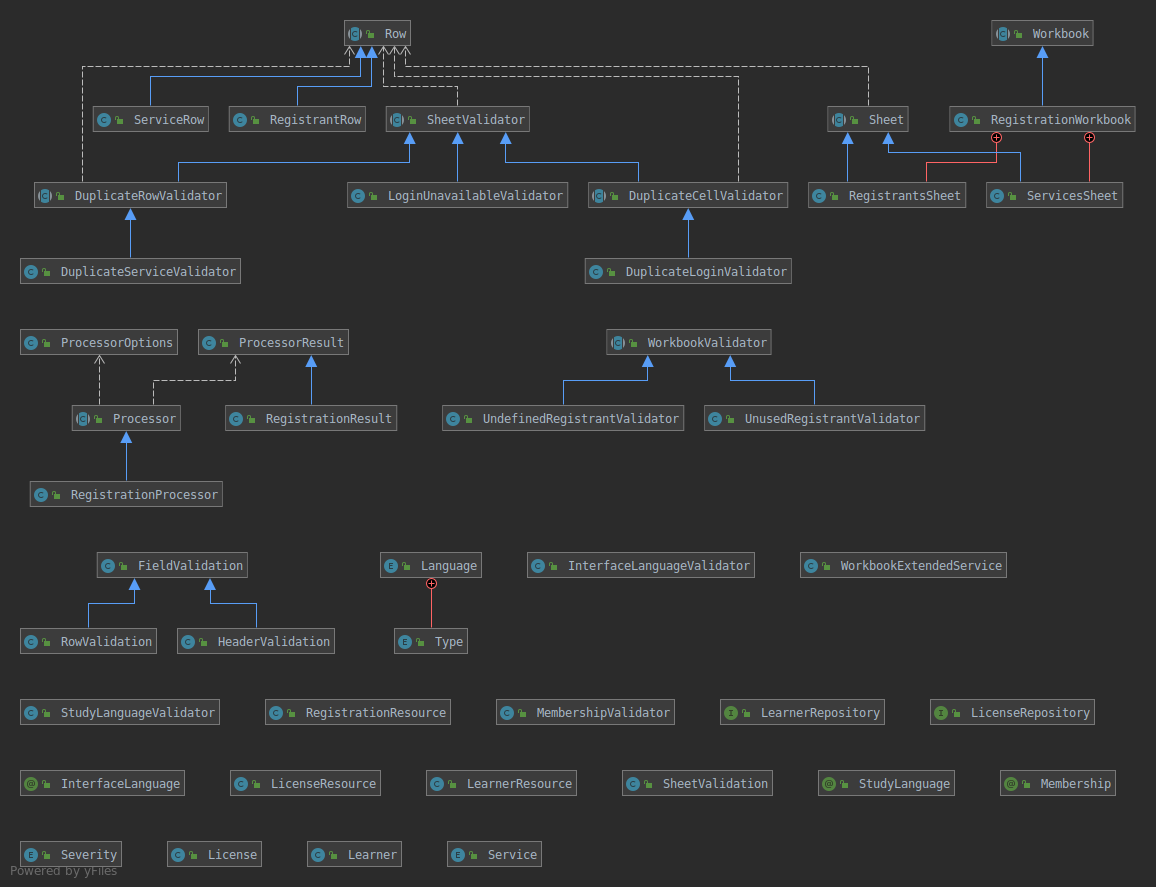
\includegraphics[width=1\textwidth]{images/diagrams/clickandrun-class-diagram.png}
    \caption{Le diagramme complet contenant les classes nécessaires à la validation et au traitement des données}
    \label{fig:class-diagram-full}
\end{figure}

\paragraph{}
Dans le diagramme \ref{fig:class-diagram-full}, on peut observer différents blocs.
Avant de passer en revue ces différents blocs, j'aimerais attirer l'attention sur la classe \lstinline{WorkbookExtendedService}.
Cette classe est de très loin la plus importante et son code est disponible en annexe \ref{ch:workbook-service-code}.

\begin{figure}[ht]
    \centering
    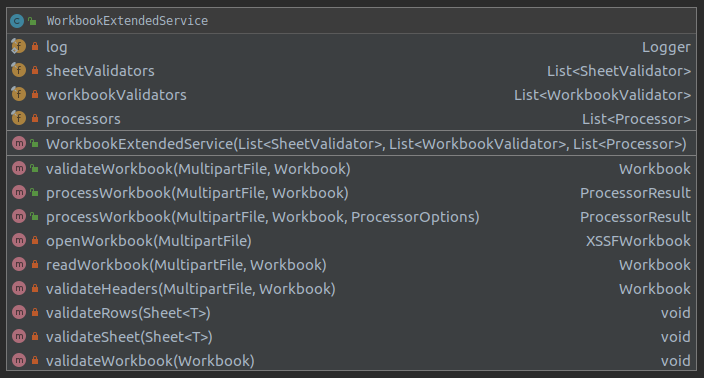
\includegraphics[width=1\textwidth]{images/diagrams/workbook-service-class.png}
    \caption{La classe qui connecte tous les bouts}
    \label{fig:class-service}
\end{figure}

\paragraph{}
Bien que cette classe soit le coeur de l'application, elle n'étend aucune classe, n'implémente aucune interface et n'est étendue par aucune classe.
Cela est possible grâce à quatre choses:
\begin{itemize}
    \item Les variables \lstinline{sheetValidators}, \lstinline{workbookValidators} et \lstinline{processors} sont toutes trois injectées par \Gls{g-spring} (voir sous-section \ref{subsubsec:dependency-injection} pour plus de détails sur l'injection de dépendances)
    \item La classe définit un paramètre générique \lstinline{T} qui peut être n'importe quelle classe qui étend la classe \lstinline{Row}
    \item Les instances de la classe \lstinline{T} sont peuplées en utilisant le mécanisme de réflexion\fnmark{}
    \fntext{Le mécanisme de réflexion est la capacité qu'un programme a à s'examiner lui-même.}
    \item Le patron de conception de la stratégie permet d'obtenir la stratégie adaptée pour traiter un objet sans connaitre cet objet.
\end{itemize}

Un paramètre générique permet d'utiliser une classe non spécifiée tout en étant capable d'utiliser ses capacités spécifiques.
Lors de l'exécution du code, \lstinline{T} pourrait en réalité être \lstinline{RegistrationWorkbook}.
La généricité n'est pas à confondre avec le polymorphisme\fnmark{}.
\fntext{Le polymorphisme est la capacité d'une fonction informatique à accepter tout paramètre qui est descendant du type attendu. Ainsi, si vous avez besoin d'un fruit, vous serez satisfait d'une banane mais vous ne pourrez pas vous servir des caractéristiques propres à la banane car vous ne savez pas que c'est une banane. Vous savez juste que c'est un fruit.}
Ce dernier ne permet pas d'accéder au comportement spécifique de l'instance manipulée.

Le mécanisme de réflexion permet d'examiner la classe non spécifiée pour comprendre son comportement.
En examinant la classe \lstinline{RegistrationWorkbook}, le programme détermine quels champs correspondent à quelles données du fichier Excel.

La patron de conception de la stratégie permet de choisir les stratégies adaptés à l'instance traitée.
Le service a reçu toutes les stratégies possibles lors de sa création.
Ces stratégies ne sont autres que les membres des variables \lstinline{sheetValidators}, \lstinline{workbookValidators} et \lstinline{processors}.
Il passe en revue toutes les stratégies une à une et elle détermine elle-même si elles sont adaptées ou non.
C'est le concept caché dernière ce patron de conception; c'est la stratégie qui définit si elle est valide ou non, et pas le service qui emploie la stratégie.

Pour être une stratégie, une classe doit implémentée une interface qui fournit deux méthodes: une qui valide la compatibilité de la stratégie et une qui applique la stratégie.
Voici l'interface d'un des trois types de stratégie:
\begin{lstlisting}[language=Java]
/**
 * Interface to define a post-validator for business / functional validation in the whole workbook
 */
public abstract class WorkbookValidator {

 protected static final Logger log = LoggerFactory.getLogger(WorkbookValidator.class);
 
 /**
  * Assert if this validator is suitable for a particular workbook
  * @param definition the definition to check
  * @return true if this validator is suitable for the provided workbook
  */
 public abstract boolean isApplicableTo(Workbook definition);
 
 /**
  * Actual validation process
  * @param workbook the workbook to add error / warning to
  * @return the number of error/warning issued by this validator
  */
 public abstract long validate(Workbook workbook);

}
\end{lstlisting}

\begin{figure}[ht]
    \centering
    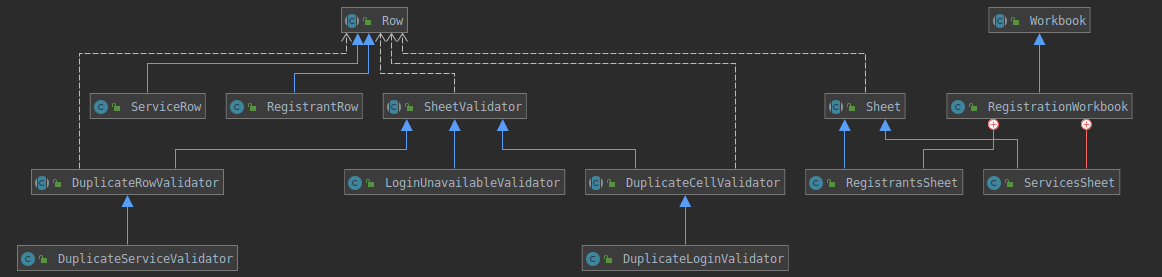
\includegraphics[width=1\textwidth]{images/diagrams/row-dependencies.png}
    \caption{Les classes liées au modèle}
    \label{fig:class-model}
\end{figure}
\paragraph{}
Le bloc repris dans la figure \ref{fig:class-model} est nettement orienté.
Tous les flèches sont dirigées vers les classes modèles du \gls{g-framework}.

Les cinq classes \lstinline{RegistrationWorkbook}, \lstinline{ServicesSheet}, \lstinline{RegistrantSheet}, \lstinline{ServiceRow} et \lstinline{RegistrantRow} constituent un module.
L'ajout d'un module nécessite l'écriture ces classes-là, plus éventuellement les stratégies non prévues par le \gls{g-framework}.

\paragraph{}
Les classes restantes n'apportent rien de fondamentalement différent de ce qui a été abordé ici et je ne les passerai donc pas en revue.

